\chapter[Databáze 2]{B4M36DS2 \\[1ex]\Large{Pojem Big Data, základní principy distribuovaného zpracování dat, typy a vlastnosti NoSQL databází}}

Na začátek trochu slovíčkaření:

\begin{itemize}
\item \textbf{Black box testing}: Nevíme, co testujeme, nevidíme dovnitř, testy stavíme na základě pravděpodobných případů používání
\item \textbf{White box testing}: Máme k dispozici kód, děláme informované testy nebo analýzu kódu
\item \textbf{Verifikace}: Testujeme, jestli to odpovídá specifikaci
\item \textbf{Validace}: Testujeme, jestli to je to, co klient chce
\item \textbf{Regrese}: Do systému zanášíme další chyby při tom, jak se ho snažíme opravit.
\item \textbf{Test coverage}: Pokrytí testů, tedy jaká část SW je otestovaná (řádky kódu, kombinace vstupů). Vyjadřuje se v procentech.
\item \textbf{Smoke test}: Základní test funkcionality
\item \textbf{Test condition}: Něco, co testujeme, třeba funkce nebo jiná část systému. 
\end{itemize}

\paragraph{V-model} V-model je model vývoje SW od návrhu po realizaci, má dvě části, tvorbu a testování. Tvorba je business model, požadavky, funkční návrh, technický návrh, implementace. Testování jsou vývojářské testy, integrační testy, systémové testy, uživatelské akceptační testy (UAT), produkční provoz. Problém je, že čím později odhalíme chybu, tím dražší je to opravit - a pokud je ve V modelu chyba v požadavcích, odhalí to až poslední testy UAT.

\paragraph{W-model} W-model je podobný V-modelu, ale opravuje chybu s pozdním odhalením chyby. Tentokrát je nějaká forma revize nebo testu přítomná v každém kroku, tedy po požadavcích, návrhu atd.

\paragraph{Quality gates} Quality Gates jsou kontroly mezi jednotlivými kroky ve fázi tvorby V/W modelu. Buď jsou striktní, tj dokud to někdo neschválí, tak se nemůže pokračovat, nebo jsou kooperativní, kdy ten, kdo práci dokončil odpovídá na otázky tomu, kdo projekt přebírá, a všichni se ujišťují, že je vše ok.

\paragraph{Statické testování} Testujeme komponentu nebo systému na úrovni specifikace nebo implementace bez spouštění systému. Probíhá v částí Tvorby ve V-modelu. Pro specifikaci se dělají různé úrovně revizí, pro implementaci se dělá Code Review a jiné statické analýzy kódu. Revize mají čtyři úrovně:

\begin{enumerate}
\item Informal review: Neformální kontrola
\item Walktrough: Autor ukazuje dílo ostatním a komentuje to
\item Technical review: Formální, někdo to moderuje (ne autor)
\item Inspection: Formální, někdo to moderuje, je předem daný proces, pořizuje se zápis, používají se metriky atd.
\end{enumerate}

\paragraph{Jak hodnotit specifikaci} Nechceme tam mít vágní formulace: \textit{by mělo}, chybějící části: \textit{tohle, tamto, atd}, nedodělky: \textit{TODO}, nakopírované kusy, chybějící odkazy na dokumentaci. Specifikaci můžeme kontrolovat tak, že ji projdeme a na základě toho sestavíme popis aplikace (ten by měl odpovídat realitě). Dělá se to v krocích, každý krok má dvě části, a totiž návrh a kontrola. V návrhu sepíšeme vše, co jsme našli, a v kontrole ověřujeme, že vše se použije, a že to dává smysl.
\begin{enumerate}
\item Zjistit, kdo jsou uživatelé
\item Zjistit, jaké funkce systém poskytuje (a komu)
\item Namapovat uživatele na funkce
\end{enumerate}



\section{Automatizace testů}

Automatizace se vyplatí, když máme opakující se testy, různé platformy, nebo chceme testovat hodně parametrů. Jde to dělat různě: klikací automat, sekvence HTTP packetů, javascript inject do stránky, pluginy pro prohlížeč, OCRka.

Taky se dají dělat jednotkové testy (česky unit testy), kde se v kódu volají funkce a zjišťuje se, jestli vrátily to, co měly, případně jestli vyhodily správnou výjimku. Unit testy by se měly vytvářet (a spouštět) průběžně během vývoje.


\section{Výběr dat}

\paragraph{Třídy ekvivalence} Máme aplikaci, která dává slevu na základě ceny nákupu: 0-499kč žádná sleva, 500-999kč 5\% sleva, 1000kč a víc 5\% sleva a doprava zdarma. Pak nemusíme testovat všechny hodnoty, ale stačí vybrat z každého rozsahu jednu hodnotu, a navíc otestovat hraniční hodnoty. Tyhle intervaly jsou naše třídy ekvivalence, protože pro hodnoty z jednoho intervalu se bude aplikace chovat stejně. Druhým typem tříd ekvivalence (kromě intervalů) jsou diskrétní hodnoty (metoda platby, typ prohlížeče atd). Třídy ekvivalence mohou být validní (to, co aplikace očekává), nebo nevalidní (místo částky je tam string, nebo je částka záporná).

\subsection{Výběr kombinace dat} Použitím tříd ekvivalence jsme se dostali na rozumný počet dat, ale když budeme testovat nějakou funkci, musíme stejně vybrat, kolik kombinací vstupu uděláme. Dá se to nakreslit jako strom (klasifikační strom), kde v kořeni je název funkce, jako děti jsou názvy vstupních parametrů, a listy jsou možné hodnoty (tedy třídy ekvivalence). Na výběr kombinace vstupů je přibližně tisíc možných postupů, ve slidech jsou všechny, ale jen některé se vysvětlují:
\begin{description}
\item[MCC - Multiple Condition Coverage] testujeme všechny možné kombinace
\item[MC/DC - Modified Condition/Decision Coverage] testujeme všechny kombinace, které mají mít odlišný výsledek	
\item[Pairwise testing] tesujeme všechny možné dvojice dat
\item[C/DC - Condition/Decision Coverage]
\item[CC - Condition Coverage]
\item[DC - Decision Coverage]
\item[Ruční výběr] ještě menšího množství kombinací
\end{description}

Čím je postup níž v seznamu, tím má horší pokrytí. Kritické aplikace používají MCC nebo MC/DC. Existuje software, který generuje testovací sady za nás.

Příklad: Máme funkci, která má rozhodnout, jestli může pilot létat zaoceánské lety, odmínka je následující: \textit{Pokud pilot (má nalétáno víc než 200 hodin nebo absolvoval víc než 10 linkových letů) a zároveň prošel výcvikem pro let nad mořem, pak může létat na zaoceánských letech}. To jde pro účely testování zkrátit jako $R = ( A \vee B ) \wedge C$.

\paragraph{MCC} Máme tři vstupy, všechny jsou binární (má/nemá nalétáno, prošel/neprošel výcvikem). Počet MCC kombinací zjistíme tak, že vynásobíme počet variant v každé proměnné, tedy v tomto případě budeme mít $2\cdot 2 \cdot 2 = 8$ testů: 000, 001, 010, 011, 100, 101, 110, 111.

\paragraph{MC/DC} Uděláme pravdivostní tabulku a z nějakého důvodu na diagonálu pro každou proměnnou dáme nějakou hodnotu (modrá čísla). Zbylé proměnné doplníme tak, aby výsledek odpovídal hodnotě ve sloupci (černá čísla nahoře). To se dělá tak, že tam dáme \textit{neutrální hodnoty} - pro AND je neutrální hodnota 1, pro OR je to 0. V~poslední řádce to jde udělat více způsoby, tak vybereme ty, které už se tam někdy vyskytují, tedy 011 a třeba 000, to druhé je jedno). Testy, které se opakují (třeba 001) děláme jen jednou. Dostali jsme tedy testy: 101, 011, 001, 000.

\begin{figure}[ht!]
\centering
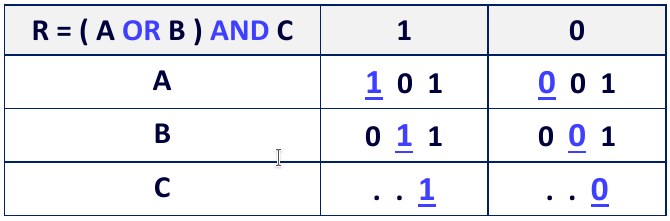
\includegraphics[width=0.5\textwidth]{ZKS/img/mcdc.png}
\end{figure}

\paragraph{Pairwise testing} Chceme vybrat každou dvojici, takže pro AB: 01, 10, 00, 11, pro BC: 01, 10, 00, 11, pro AC: 01, 10, 00, 11. To splňuje třeba sada testů: 000, 011, 110, 101. 


\section{Testy průchodu}

\paragraph{Free testing} Nevíme, jak aplikace funguje, nějak tím klikáme a zkoušíme

\paragraph{Exploratory testing} Jako free testing, ale zaznamenáváme, co jsme zkoušeli

\subsection{Pokrytí cest}

Když víme, jak aplikace funguje, tak vycházíme z vývojového diagramu. Ten si nakreslíme a popíšeme body a hrany. Pak zvolíme hloubku testu (pokrytí cest):

\begin{itemize}
\item Hloubka 1: Projdeme každou hranu aspoň jednou
\item Hloubka 2: Projdeme každou dvojici po sobě následujících hran aspoň jednou (tedy v každém bodě vyzkoušíme všechny kombinace vstupu a odchodu).
\item Hloubka 3: Projdeme každou trojici po sobě následujících hran aspoň jednou.
\end{itemize}

Pak sestavíme testy tak, abychom jich měli co nejméně, a přesto jsme pokryli všechny průchody s požadovanou hloubkou. Další možnost je \textit{Elementary comparison test}, kdy zkoušíme průchody a kombinace dat zároveň. V některých postupech (PA a ST - smoketest) se navíc pracuje s prioritami, tedy pokud si můžeme vybrat, kterou hranu projdeme víckrát, vybereme tu s vyšší prioritou.

\subsection{Konzistence dat}

Testování dle pokrytí nemusí být dostatečné pro chyby, které se týkají dat. Jedna část kódu může data poškodit, a jiná je pak nebude moci použít - přitom takový průchod vůbec nemusel být testován, i když budeme mít otestované pokrytí cest. Manipulace s daty má 4 kroky: create, read, update, delete, a říká se tomu CRUD.

Práci aplikace s daty v aplikaci se sepíše do CRUD matice, což je tabulka, kde je pro každý druh dat (objekt?) a každou funkci napsané, jaká operace se s danými daty v dané funkci dělá. Obvykle by každý objekt měl být někde vytvořen, přečten, a následně smazán, ale pokud to tak není, nevadí to, v některých případech by to nedávalo smysl.

Pro každý objekt sestavíme několik scénářů, jak se s objektem v aplikaci pracuje: typicky vytvoření, pak kombinace čtení a úprav, a pak smazání. Sestavíme posloupnost funkcí, kde se tyto akce s objektem dělají. Pak testujeme průchody aplikací tak, abychom volali ty správné funkce.